% --- Configuration ------------------------------------------------------
% add shortcut for github url of this chapter
\def \GITHUB {\GITHUBBASE/01_introduction}
% add the fig folders
\graphicspath{%
{\PATH/\CHAPONE/}%
{\PATH/\CHAPONE/fig1_01/}%
}

% --- Document -----------------------------------------------------------
\chapter{Introduction}
\label{cha:introduction}
%
Write a general introduction to this document.
%
\section{Reproducible Research}
\label{sec:reproducible_research}
%
Like other fields that involve signal processing, the study of \ac{SFS}
implies implementing a multitude of algorithms and running numerical simulations
on a computer
As a consequence, the outcome of the algorithms are easily vulnerable to
implementation errors which cannot completely be
avoided.\sidenote[][-1.5cm]{\cite[Compare][]{Ince2012}}

Beside the software tools, the work presented here relies on measured acoustical
data.
To ensure that other
researchers can test the correctness of results and easily reproduce them,
the most straightforward approach is to publish the code together with the
measured data.
This policy was adapted in the last years by some journals and is known under the
term \emph{reproducible research}.\sidenote[][-2.7cm]{\cite[For one of the pioneers
see][]{Donoho2009}}
It is included in this document as well.
Functions derived in the theoretical chapter that are implemented in the
toolbox are accompanied by a link to the corresponding function. All figures in
this document have a link in the form of \reproduce{\GITHUBBASE} which is a link to a
folder containing all the data and scripts in order to reproduce the single
figures.


%%%%%%%%%%%%%%%%%%%%%%%%%%%%%%%%%%%%%%%%%%%%%%%%%%%%%%%%%%%%%%%%%%%%%%%%%%%%%%%%
\section{Mathematical Definitions}
\label{sec:mathematical_definitions}
%
\begin{figure}
    \centering
    \small
    % GNUPLOT: LaTeX picture with Postscript
\begingroup
  \makeatletter
  \providecommand\color[2][]{%
    \GenericError{(gnuplot) \space\space\space\@spaces}{%
      Package color not loaded in conjunction with
      terminal option `colourtext'%
    }{See the gnuplot documentation for explanation.%
    }{Either use 'blacktext' in gnuplot or load the package
      color.sty in LaTeX.}%
    \renewcommand\color[2][]{}%
  }%
  \providecommand\includegraphics[2][]{%
    \GenericError{(gnuplot) \space\space\space\@spaces}{%
      Package graphicx or graphics not loaded%
    }{See the gnuplot documentation for explanation.%
    }{The gnuplot epslatex terminal needs graphicx.sty or graphics.sty.}%
    \renewcommand\includegraphics[2][]{}%
  }%
  \providecommand\rotatebox[2]{#2}%
  \@ifundefined{ifGPcolor}{%
    \newif\ifGPcolor
    \GPcolortrue
  }{}%
  \@ifundefined{ifGPblacktext}{%
    \newif\ifGPblacktext
    \GPblacktextfalse
  }{}%
  % define a \g@addto@macro without @ in the name:
  \let\gplgaddtomacro\g@addto@macro
  % define empty templates for all commands taking text:
  \gdef\gplbacktext{}%
  \gdef\gplfronttext{}%
  \makeatother
  \ifGPblacktext
    % no textcolor at all
    \def\colorrgb#1{}%
    \def\colorgray#1{}%
  \else
    % gray or color?
    \ifGPcolor
      \def\colorrgb#1{\color[rgb]{#1}}%
      \def\colorgray#1{\color[gray]{#1}}%
      \expandafter\def\csname LTw\endcsname{\color{white}}%
      \expandafter\def\csname LTb\endcsname{\color{black}}%
      \expandafter\def\csname LTa\endcsname{\color{black}}%
      \expandafter\def\csname LT0\endcsname{\color[rgb]{1,0,0}}%
      \expandafter\def\csname LT1\endcsname{\color[rgb]{0,1,0}}%
      \expandafter\def\csname LT2\endcsname{\color[rgb]{0,0,1}}%
      \expandafter\def\csname LT3\endcsname{\color[rgb]{1,0,1}}%
      \expandafter\def\csname LT4\endcsname{\color[rgb]{0,1,1}}%
      \expandafter\def\csname LT5\endcsname{\color[rgb]{1,1,0}}%
      \expandafter\def\csname LT6\endcsname{\color[rgb]{0,0,0}}%
      \expandafter\def\csname LT7\endcsname{\color[rgb]{1,0.3,0}}%
      \expandafter\def\csname LT8\endcsname{\color[rgb]{0.5,0.5,0.5}}%
    \else
      % gray
      \def\colorrgb#1{\color{black}}%
      \def\colorgray#1{\color[gray]{#1}}%
      \expandafter\def\csname LTw\endcsname{\color{white}}%
      \expandafter\def\csname LTb\endcsname{\color{black}}%
      \expandafter\def\csname LTa\endcsname{\color{black}}%
      \expandafter\def\csname LT0\endcsname{\color{black}}%
      \expandafter\def\csname LT1\endcsname{\color{black}}%
      \expandafter\def\csname LT2\endcsname{\color{black}}%
      \expandafter\def\csname LT3\endcsname{\color{black}}%
      \expandafter\def\csname LT4\endcsname{\color{black}}%
      \expandafter\def\csname LT5\endcsname{\color{black}}%
      \expandafter\def\csname LT6\endcsname{\color{black}}%
      \expandafter\def\csname LT7\endcsname{\color{black}}%
      \expandafter\def\csname LT8\endcsname{\color{black}}%
    \fi
  \fi
  \setlength{\unitlength}{0.0500bp}%
  \begin{picture}(4534.00,2834.00)%
    \gplgaddtomacro\gplbacktext{%
      \csname LTb\endcsname%
      \put(254,1125){\makebox(0,0){\strut{}$z$}}%
      \colorrgb{0.65,0.81,0.89}%
      \put(1320,687){\makebox(0,0)[l]{\strut{}$\phi$}}%
      \put(1318,955){\makebox(0,0)[l]{\strut{}$\theta$}}%
      \colorrgb{0.12,0.47,0.71}%
      \put(2629,2070){\makebox(0,0)[l]{\strut{}\vec{x}}}%
    }%
    \gplgaddtomacro\gplfronttext{%
      \csname LTb\endcsname%
      \put(2166,240){\makebox(0,0){\strut{}$x$}}%
      \put(761,1449){\makebox(0,0){\strut{}$y$}}%
      \put(254,1125){\makebox(0,0){\strut{}$z$}}%
    }%
    \gplbacktext
    \put(0,0){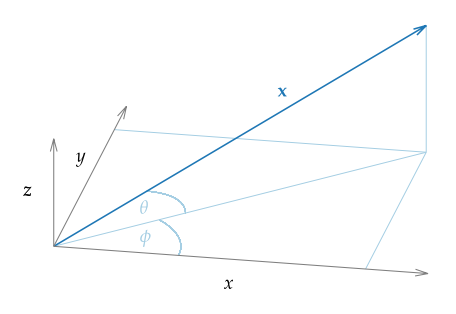
\includegraphics{coordinate_system}}%
    \gplfronttext
  \end{picture}%
\endgroup

    \caption{Coordinate system used in this thesis. The vector $\vec{x}$ can also
    be described by its length, its azimuth angle $\phi$, and its elevation
    $\theta$.
    \reproduce{\GITHUB/fig1_01}}
    \label{fig:coordinate_system}
\end{figure}
%
\paragraph{Coordinate system}
Figure\,\ref{fig:coordinate_system} shows the coordinate system that is used in
the following chapters. A vector $\vec{x}$ can be described by its position
$(x,y,z)$ in space or by its length, azimuth angle $\phi \in [0,2\PI[$,
and elevation $\theta \in \left[-\frac{\PI}{2},\frac{\PI}{2}\right]$.
The azimuth is measured counterclockwise and elevation is positive
for positive $z$-values.


%----%----%----%----%----%----%----%----%----%----%----%----%----%----%----%----
\paragraph{Fourier transformation}
Let $s$ be an absolute integrable function, $t,\omega$ real numbers, then the
temporal Fourier transform is defined as\autocite{Bracewell2000}
%
\begin{equation}
    S(\omega) = \FT{s(t)} = \int^{\infty}_{-\infty} s(t) \E^{-\I\omega t}
    \; \D{t}
    \qp
    \label{eq:ft}
\end{equation}

In the same way the inverse temporal Fourier transform is defined as
%
\begin{equation}
    s(t) = \IFT{S(\omega)} = \frac{1}{2\PI} \int^{\infty}_{-\infty} S(\omega)
    \E^{\I\omega t} \; \D\omega
    \qp
    \label{eq:ift}
\end{equation}
